\section{Análisis y discusión de los resultados}

Con el objetivo de observar la relación entre el valor F1 alcanzado y la magnitud $n$ en el conjunto de datos, se presentan la figuras \ref{fig:aumento_n_depresion}, \ref{fig:aumento_n_depresion19} y \ref{fig:aumento_n_anorexia}. En las gráficas se comparan los métodos: sin aumento de datos, Tesauro, restricción $\chi^2$ , relación equivalente y relación contraria. Las gráficas se presentan en una escala de 0 a 100\% para el valor $F1$, el eje $x$ refleja el número de secuencias aumentadas por cada secuencia original en ele conjunto de entrenamiento y el eje $y$ la ganancia o perdida en $F1$ en comparación con la línea base que es no realizar aumento de datos. 

En la figura \ref{fig:aumento_n_depresion} (a), el aumento para la red bidireccional, el mejor resultado con una ganancia de 4.51 puntos se obtiene con $n=4$ con el método \textit{Restricción $\chi^2$}. Se puede observar que una vez alcanzado el balance la ganancia comienza a decrecer, los métodos restantes no obtienen la misma ganancia, por lo que en esta tarea es importante conservar las características discriminantes cuando se realiza el aumento de datos, sin embargo, si el conjunto se n-plica muchas veces el modelo se sobre ajusta a los datos que se conservan.

En la figura \ref{fig:aumento_n_depresion} (b), aumento de datos para la red CNN, el mejor valor encontrado con una ganancia de 5.45 puntos fue con $n=6$ con el método \textit{Restricción $\chi^2$}. A diferencia de la red recurrente las ganancias en F1 se encuentran en un rango entre 0 y 5 puntos, los métodos con menor ganancia fueron; el basado en equivalencias y el relaciones contrarias.

En la figura \ref{fig:aumento_n_depresion} (c), aumento de datos para SVM, se presenta una tendencia creciente en relación al parámetro $n$, el mejor valor obtenido es una ganancia de 38 puntos mediante el método \textit{Restricción $\chi^2$}. En este caso la ganancia se debe más a la afectación de los pesos \textit{tf-idf} que al aumento de datos, aún así el método basado en restricción $\chi^2$ ofrece una mejora desde el primer documento en comparación con los otros métodos. La figura \ref{fig:aumento_n_depresion} (d) representa los resultados en el algoritmo SVM-C, esta figura muestra que el aumento de datos en este caso no es necesario para este tipo de modelos o no se aprovecha como lo haría una red neuronal.

Las gráficas que representan la comparación de los algoritmos propuestos para el conjunto de datos Depresión 2019, se presenta en la figura \ref{fig:aumento_n_depresion19}. En la subfigura (a) la única ganancia significativa se da en el modelo Bi-LSTM con 13.82 puntos en \textit{F1}, sin embargo después de triplicar conjunto de entrenamiento para la clase positiva ocurre lo contrario. Estas variaciones muy notables se deben a que el conjunto de test es menor y por lo tanto los falsos positivos afectan en gran medida en la evaluación. En la subfigura (b) se presenta la evaluación en el modelo CNN, en este caso el método del estado del arte Tesauro obtiene mejores resultados en comparación con los métodos propuestos. En la subfigura (c) aumentar el conjunto mediante relaciones contrarias obtiene mejores resultados, aunque se le puede atribuir al peso que se le asigna a las palabras, dado que el método de relaciones contrarias aumenta documentos de clase positiva para aumentar la clase positiva. Su contra parte se representa en la subfigura (d)  y dado que el algoritmo SVM-C considera el desbalance de los ejemplos no se consiguen mejoras. Como nota final en este conjunto no se consigue el balance de clases debido a las proporciones del conjunto.


La figura \ref{fig:aumento_n_anorexia} presenta el aumento de datos para el conjunto de anorexia. Al igual que en las gráficas anteriores se presenta el efecto del aumento de datos en los diferentes algoritmos de clasificación empleados. Similar que en los conjuntos de depresión el método de Restricción $\chi^2$ obtiene mejores ganancias en los diferentes aumentos. Para la red convolucional la ganancia es menor, pero se observa que es el método más consistente ya que los diferentes aumentos no afectan en sentido contrario a la clasificación como sucede con el método de tesauro y equivalencia contraria. Para el modelo lineal SVM el método de equivalencias contrarias obtiene mejores resultados, conforme crece el aumento de datos pero en el modelo SVM-C obtiene el peor rendimiento. Para el modelo SVM-C el método de Restricción $\chi^2$ vuelve a sobre salir con hasta 4.98 puntos de ganancia a la línea base, acumulando más evidencia sobre nuestra hipótesis inicial.


%\newpage

\begin{figure}[hbt!]
    \begin{subfigure}[b]{0.5\textwidth}
        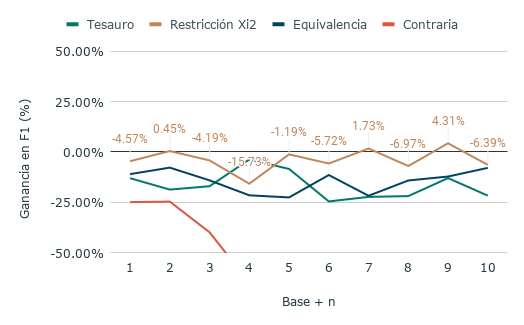
\includegraphics[width=\textwidth]{sections/figures/bi_LSTM2018.png}
        \caption{Bi-LSTM}
    \end{subfigure}
    \hfill
    \begin{subfigure}[b]{0.5\textwidth}
        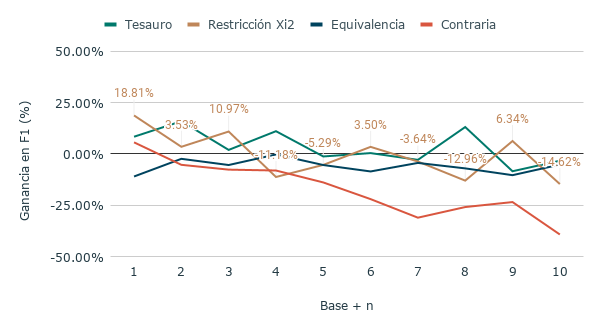
\includegraphics[width=\textwidth]{sections/figures/CNN2018.png}
        \caption{CNN}
    \end{subfigure}
    
  
    % \begin{subfigure}[b]{0.5\textwidth}
    %     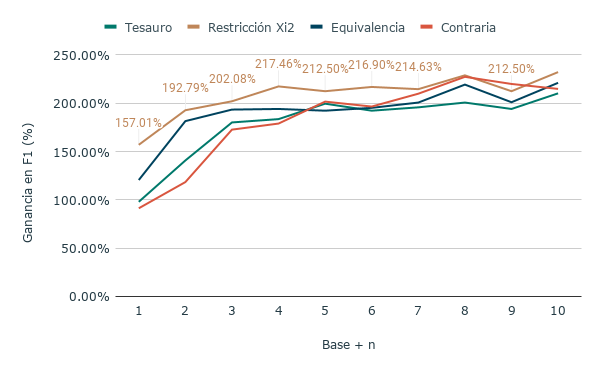
\includegraphics[width=\textwidth]{sections/figures/SVM2018.png}
    %     \caption{SVM}
    % \end{subfigure}
    % \hfill
    % \begin{subfigure}[b]{0.5\textwidth}
    %     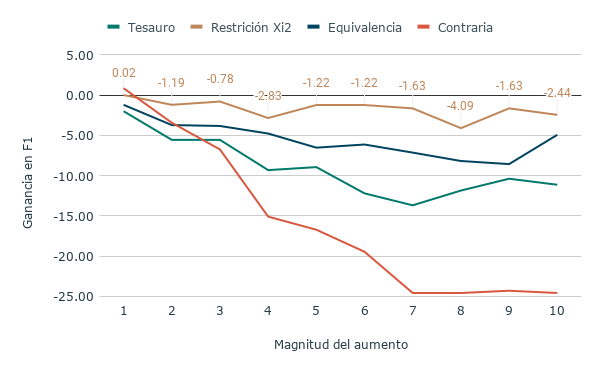
\includegraphics[width=\textwidth]{sections/figures/SVM-C2018.png}
    %     \caption{SVM-C}
    % \end{subfigure}

   
    \caption{Relación entre el aumento del conjunto de datos \textit{Depresión 2018} y la ganancia porcentual en F1.}
    \label{fig:aumento_n_depresion}
\end{figure}


\newpage
\begin{figure}[hbt!]
    \begin{subfigure}[b]{0.5\textwidth}
        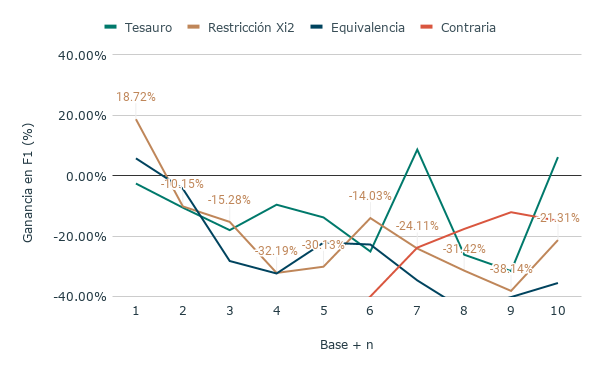
\includegraphics[width=\textwidth]{sections/figures/bi_LSTM2019.png}
        \caption{Bi-LSTM}
    \end{subfigure}
    \hfill
    \begin{subfigure}[b]{0.5\textwidth}
        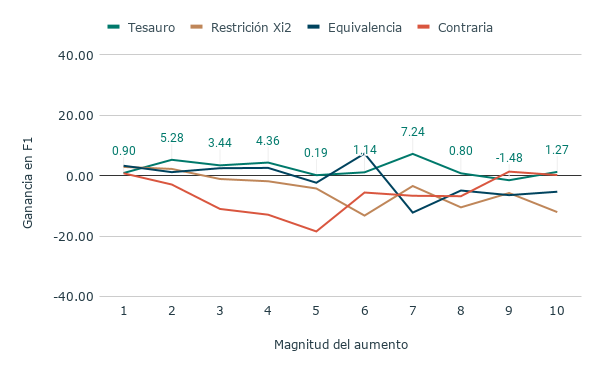
\includegraphics[width=\textwidth]{sections/figures/CNN2019.png}
        \caption{CNN}
    \end{subfigure}
    
  
    % \begin{subfigure}[b]{0.5\textwidth}
    %     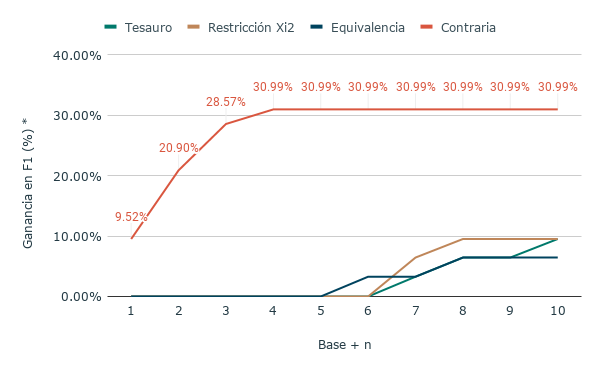
\includegraphics[width=\textwidth]{sections/figures/SVM2019.png}
    %     \caption{SVM}
    % \end{subfigure}
    % \hfill
    % \begin{subfigure}[b]{0.5\textwidth}
    %     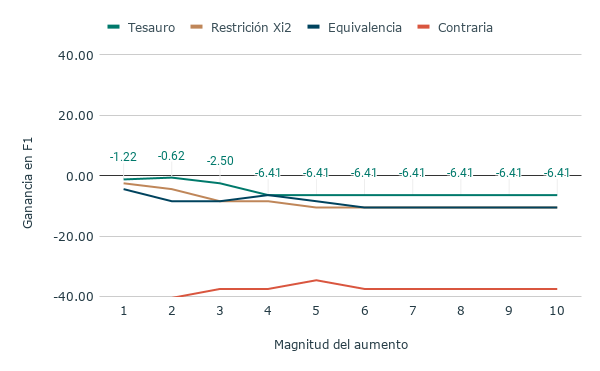
\includegraphics[width=\textwidth]{sections/figures/SVM-C2019.png}
    %     \caption{SVM-C}
    % \end{subfigure}

   
    \caption{Relación entre el aumento del conjunto de datos \textit{Depresión 2019} y la ganancia porcentual en F1.}
    \label{fig:aumento_n_depresion19}
\end{figure}


\newpage
\begin{figure}[hbt!]
    \begin{subfigure}[b]{0.5\textwidth}
        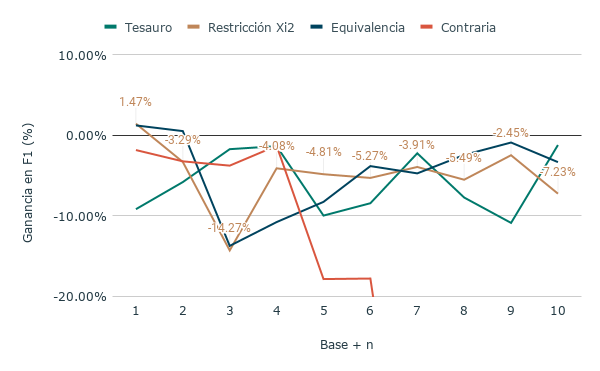
\includegraphics[width=\textwidth]{sections/figures/bi_LSTMAnox.png}
        \caption{Bi-LSTM}
    \end{subfigure}
    \hfill
    \begin{subfigure}[b]{0.5\textwidth}
        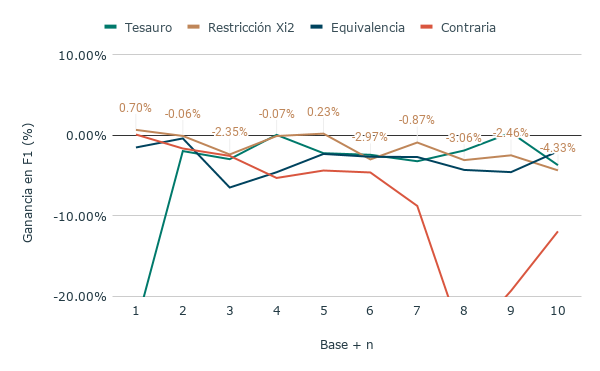
\includegraphics[width=\textwidth]{sections/figures/CNNAnox.png}
        \caption{CNN}
    \end{subfigure}
    \hfill
    
    

    % \begin{subfigure}[b]{0.5\textwidth}
    %     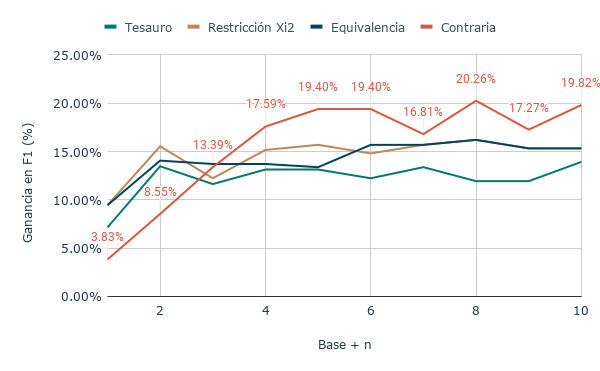
\includegraphics[width=\textwidth]{sections/figures/SVMAnox.png}
    %     \caption{SVM}
    % \end{subfigure}
    % \begin{subfigure}[b]{0.5\textwidth}
    %     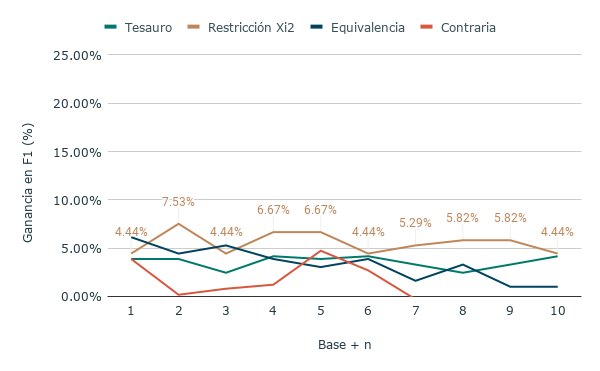
\includegraphics[width=\textwidth]{sections/figures/SVM-CAnox.png}
    %     \caption{SVM-C}
    % \end{subfigure}
    
    \caption{Relación entre el aumento del conjunto de datos \textit{Anorexia} y la ganancia porcentual en F1.}
    \label{fig:aumento_n_anorexia}
\end{figure}
\newpage

\subsection{Comparación con el estado del arte en detección de depresión y anorexia}
En la figura \ref{fig:state_of_art} se comparan los resultados obtenidos mediante aumento de datos utilizando una red Bi-LSTM y el aumento de datos mediante el método Restrición $\chi^2$, con los modelos evaluados en la conferencia eRISK 2018 \citep{Losada2018}. Para detección de depresión de un total de 45 modelos nuestra propuesta se puede ubicar en el sexto lugar por arriba del tercer cuartil. Para la detección de anorexia, de un total de 35 propuestas nuestro modelo quedaría en el segundo lugar y muy por encima del tercer cuartil. Es importante señalar que para la detección de depresión el mejor modelo presentado en la tarea eRisk2018 se obtuvo mediante la ingeniería de características y para la detección de anorexia se utilizó una red convolucional con vectores distribucionales entrenados en un corpus perteneciente al dominio, por lo que dichas propuestas podrían mejorar mediante el aumento de datos propuesto. Como nota final los resultados para el conjunto de Depresión 2019 no se comparan con los obtenidos en el evento eRisk2019 por que se realizo una evalución diferente.



\begin{figure}[!ht]
    \centering
  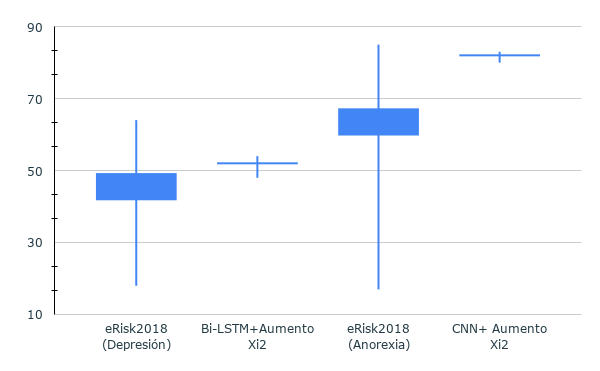
\includegraphics[scale=0.9]{sections/figures/sticks-state.png}
    \caption{Comparación con el estado del arte en detección de depresión y anorexia}
    \label{fig:state_of_art}
\end{figure}
%Poner una tabla comparativa 


\subsection{Análisis del aumento de datos}
Con el objetivo de comprobar como afecta el aumento de datos a la originalidad y diversidad del documento original, se recopilaron estadísticas del aumento en el vocabulario además de presentar las palabras más relevantes utilizadas por el método de Restrición $\chi^2$ y para el filtro de secuencias en el pre-procesamiento.

\subsubsection{Aumento del vocabulario}
En la figura \ref{fig:aumento_vocab_dep} se representa para el eje $y$ el numero de palabras nuevas agregadas en relación con el parámetro $n$ que indica la magnitud del aumento de datos. El objetivo de esta figura es comparar el vocabulario nuevo introducido de acuerdo a cada método de aumento en los diferentes conjuntos de datos.

Como se puede esperar conforme aumenta el número de documentos el vocabulario también lo hace. En las subfiguras (a, c y e) se compara el aumento del vocabulario para la clase positiva, en la cual el método basado en relaciones contrarias incrementa drásticamente el vocabulario desde un documento por cada instancia y el que menos agrega palabras es el basado en tesauro, debido a que el método tesauro utiliza el parámetro $p$ para selección igual a 0.5 y en promedio solo remplaza 2 palabras por cada segmento a aumentar. Los métodos con y sin restricción agregan el mismo número de palabras debido a que solo difieren en que palabras reemplazar. Por otra parte el basado en relaciones de equivalencia agrega un mayor vocabulario a los dos anterior por lo que se logra el objetivo de insertar un vocabulario diferente al emplear un criterio de similitud diferente.

En la subfiguras \ref{fig:aumento_vocab_dep} (b, d y f), se compara el aumento del vocabulario considerando ambas clases, debido a que el aumento de datos propuesto se basa sobre la clase de interés (la clase positiva). Resalta el hecho de que aunque el método de equivalencias contrarias introduce un gran vocabulario en la clase positiva para el conjunto de depresión 2018 y anorexia, solo agrega de 500 a 2000 mil palabras nuevas considerando ambas clases, sin embargo para el conjunto de depresión 2019 agrega hasta 7000 palabras nuevas. Este incremento drastico en el vocabulario impacta de forma negativa a los resultados. 

En resumen el método que agregó más vocabulario fue el basado en relaciones contrarias, seguido del basado en equivalencias; el método Tesauro es muy conservador en el numero de palabras nuevas agregadas pero se puede observar que las palabras agregadas no aparecen en la clase contraria. Es interesante que el método con restricción agrega la misma modificación que el que no la realiza y puede obtener mejores resultados, por lo que se comprueba la efectividad del método. 

\begin{figure}[hbt!]
    \begin{subfigure}[b]{0.5\textwidth}
        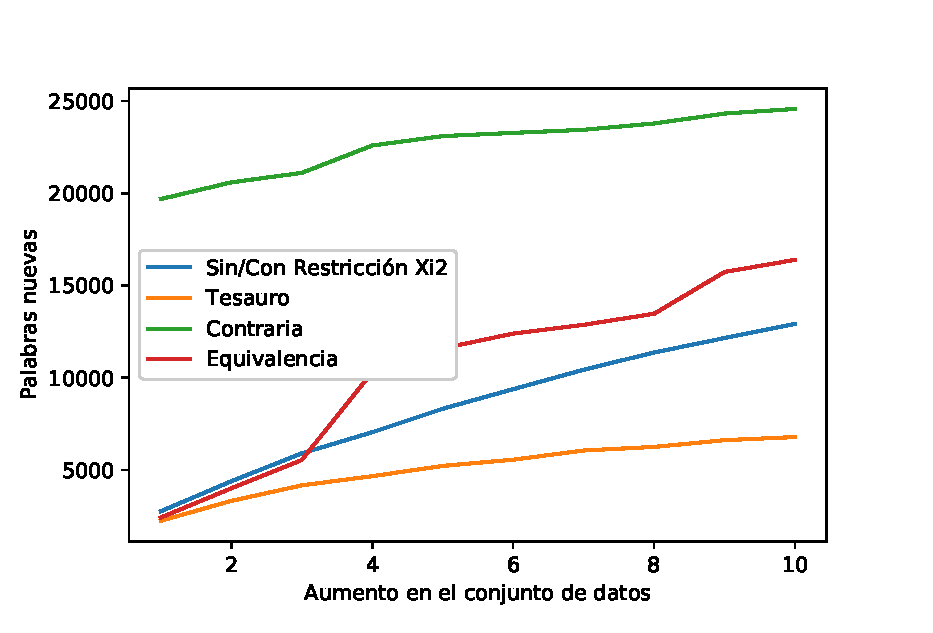
\includegraphics[width=\textwidth]{sections/figures/pos_2018.eps}
        \caption{Depresión 2018: Clase positiva}
    \end{subfigure}
    \hfill
    \begin{subfigure}[b]{0.5\textwidth}
        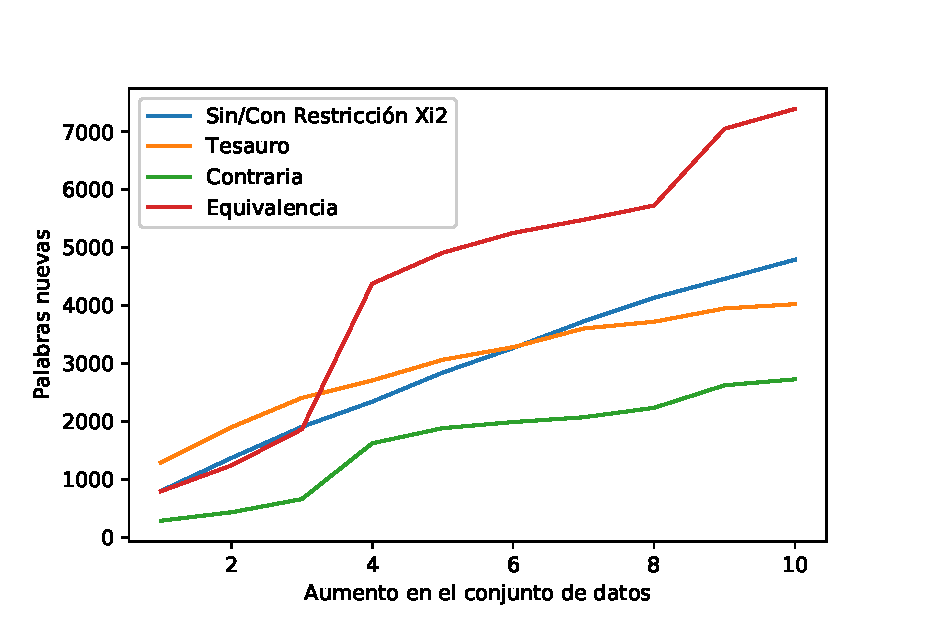
\includegraphics[width=\textwidth]{sections/figures/both2018.eps}
        \caption{Depresión 2018: Ambas clases}
    \end{subfigure}
    \hfill
    \begin{subfigure}[b]{0.5\textwidth}
        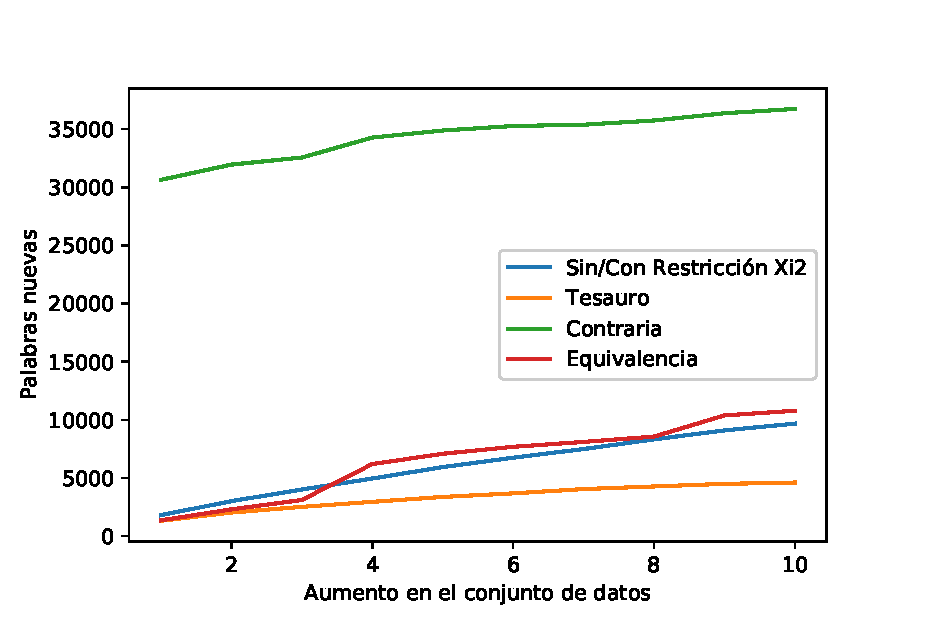
\includegraphics[width=\textwidth]{sections/figures/pos2019.eps}
        \caption{Depresión 2019: Clase positiva}
    \end{subfigure}
    \hfill
    \begin{subfigure}[b]{0.5\textwidth}
        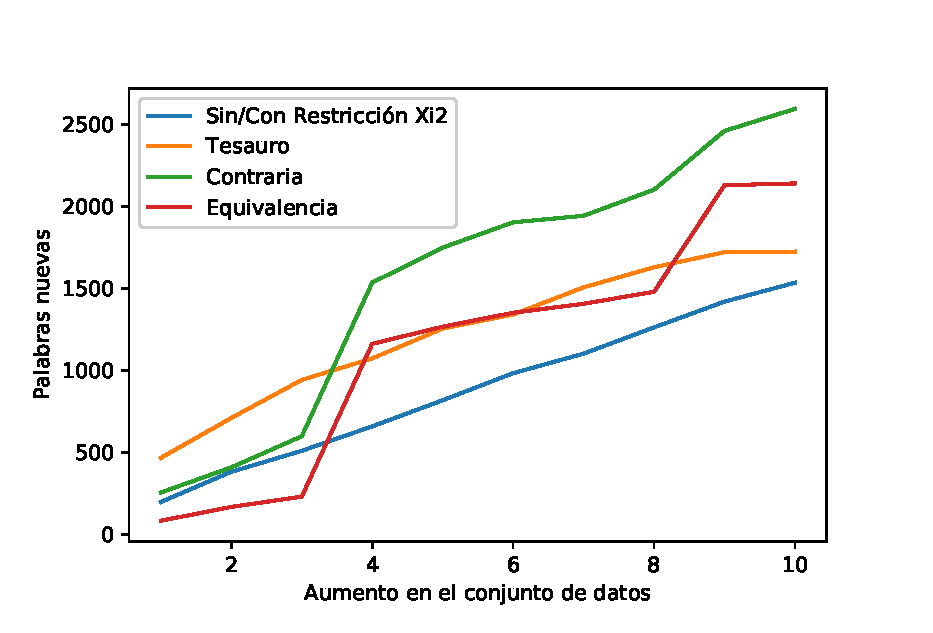
\includegraphics[width=\textwidth]{sections/figures/both2019.eps}
        \caption{Depresión 2019: Ambas clases}
    \end{subfigure}
    
    \begin{subfigure}[b]{0.5\textwidth}
        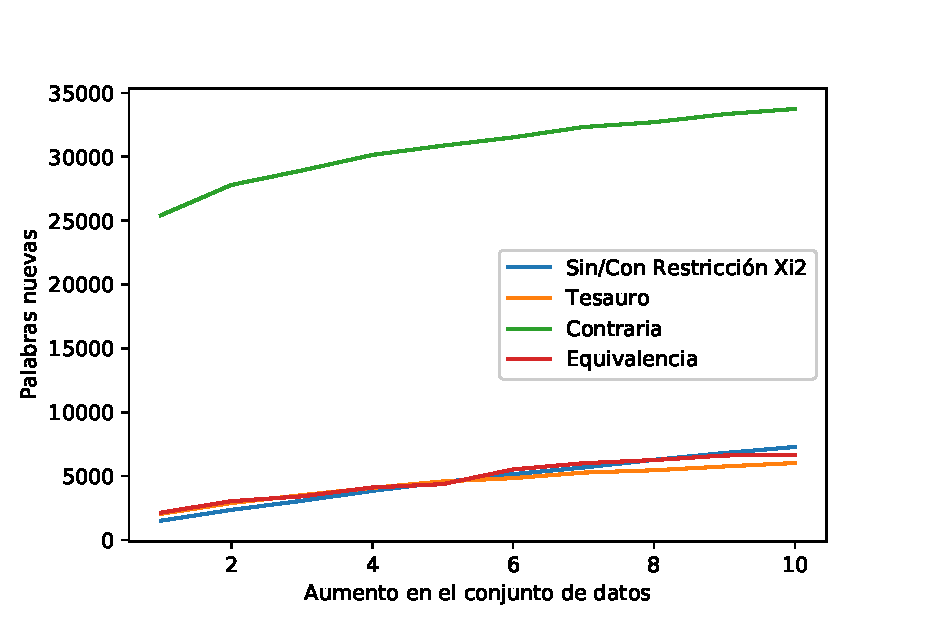
\includegraphics[width=\textwidth]{sections/figures/pos_anox.eps}
        \caption{Anorexia: Clase positiva}
    \end{subfigure}
    \hfill
    \begin{subfigure}[b]{0.5\textwidth}
        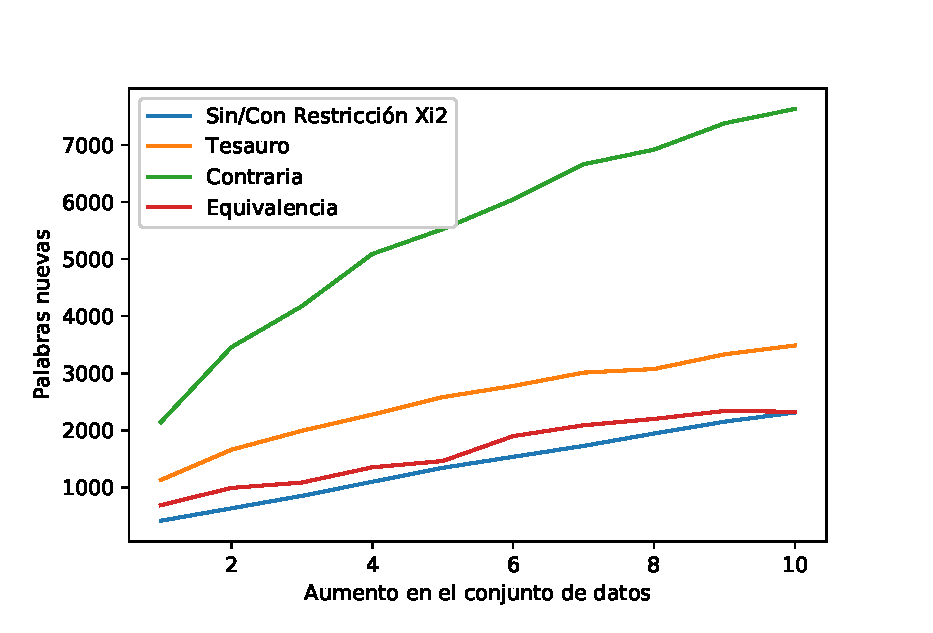
\includegraphics[width=\textwidth]{sections/figures/both_anox.eps}
        \caption{Anorexia: Ambas clases}
    \end{subfigure}
    
    
    \caption{Relación entre el aumento de datos y el vocabulario nuevo agregado.}
    \label{fig:aumento_vocab_dep}
\end{figure}

\subsubsection{Palabras con mayor puntuación $\chi^2$}
En la figura \ref{fig:words_chi_anox}, se representan las palabras con mayor puntuación $\chi^2$ mismas que sirvieron para realizar el pre-procesamiento y también para el método de aumento con restricción. La figura muestra las palabras más importantes en un tamaño de fuente más grande seguidas de las de menor importancia en una fuente más pequeña. 

Como se ha demostrado en estudios previos las palabras relacionadas con pronombres personales y posesivos son más utilizadas por personas con signos de depresión o anorexia, además de palabras relacionadas a relaciones personales como: ``boyfriend", ``feeling", ``friends", ``dating". También sobre salen palabras relacionadas a la enfermedad como: ``meds", ``medication", ``anorexia", ``depression"; entre otras.

\begin{figure}[hbt!]
\centering
 \begin{subfigure}[b]{0.7\textwidth}
        \includegraphics[width=\textwidth]{sections/figures/chi2_words_anorexia.eps}
        \caption{Anorexia}
\end{subfigure}
\hfill
\hfill
 \begin{subfigure}[b]{0.7\textwidth}
        \includegraphics[width=\textwidth]{sections/figures/chi2_words_depresion.eps}
        \caption{Depresión}
\end{subfigure}
  
    \caption{Palabras con mayor puntuación $\chi^2$}
    \label{fig:words_chi_anox}
\end{figure}


%\subsection{Relación entre precisión y recuerdo}

%\subsection{Errores}

%\subsubsection{Tipo I: Falsos positivos}

%\subsubsection{Tipo II: Falsos negativos}